\documentclass[landscape,paperwidth=50in,paperheight=34in]{baposter}

\usepackage{graphicx}
\usepackage{enumitem}
\usepackage{url}
\usepackage{tikz}
\usepackage{xcolor}

% This prevents a \section being created for the bibliography
\renewcommand{\section}[2]{}%

\newcommand{\BI}{\begin{itemize}[itemsep=.05in,parsep=0in,leftmargin=.2in]}
\newcommand{\EI}{\end{itemize}}

\newcommand{\BE}{\begin{enumerate}[itemsep=.05in,parsep=0in,leftmargin=.2in]}
\newcommand{\EE}{\end{enumerate}}

\newsavebox{\hcii}

\definecolor{paleyellow}{HTML}{FFFACD}

\tikzstyle{bigurl} = [fill=paleyellow, text=black, draw=blue, very thick, rounded corners, inner sep=8pt, inner ysep=6pt]

\begin{document}

\sbox{\hcii}{
\begin{minipage}{2.5in}
\small Human-Computer Interaction Institute,\\
Carnegie-Mellon University
\end{minipage}
}

\begin{poster}{
  % key=value Options
  columns=5,
  headerheight=0.105\textheight,
  background=plain,
  bgColorOne=white,
  borderColor=black,
  headerColorOne=blue!20!white,
  headerColorTwo=blue!20!white,
  headershape=rounded,
  headerborder=none,
  headerfont=\Large\bf,
  textborder=none,
  boxshade=none
}{
  % Eye catcher

}{
  % Poster title
   %CloudCoder: Building a Community for Using and Sharing Programming Exercises
   {\huge CloudCoder: Building a Community for Using and Sharing Programming Exercises}
}{
  % Poster authors
\vskip .05in
\hskip .25in\begin{minipage}[t]{1.3in}
{\large Jaime Spacco\\
\vskip -.2in\large Andrei Papancea\\
\vskip -.25in\small Knox College}
\end{minipage}
\begin{minipage}[t]{1.2in}
{\large Matthew Hertz\\
\vskip -.25in\small Canisius College}
\end{minipage}
\begin{minipage}[t]{1.4in}
{\large Paul Denny\\
\vskip -.25in\small University of Auckland}
\end{minipage}
\begin{minipage}[t]{1.8in}
{\large David Hovemeyer\\
\vskip -.25in\small York College of Pennsylvania}
\end{minipage}
\begin{minipage}[t]{2.5in}
{\large Kelly Rivers\\
\vskip -.2in\large John Stamper\\
\vskip -.16in\hskip -.05in\usebox{\hcii}}
\end{minipage}
}{
  % University logo(s)
  
\includegraphics[height=.5in]{images/KnoxLogo}
  \hskip .1in
  
\includegraphics[height=.5in]{images/Canisius}
  \hskip .1in
  
\includegraphics[height=.5in]{images/UniversityOfAuckland}
  \hskip .1in
  
\includegraphics[height=.5in]{images/YCPLogo}
  \hskip .1in
  
\includegraphics[height=.5in]{images/HCII_logo}
}

  % Definition of boxes
  \headerbox{tl;dr}{name=tldr,column=0}{
    \vskip .1in
    {\raggedright\normalsize
    \BI
    \item CloudCoder is a free, open-source,
          web-based {\bf programming exercise system}
    \item {\bf Multiple languages}: C/C++, Java, Python, Ruby
    \item It has a {\bf repository of free exercises}
          (contributions welcome)
    \item Ask us for a {\bf demo server account}
    \item Did we mention that it's {\bf free}?
    \EI
    }
    \vskip -.05in
    \centerline{
      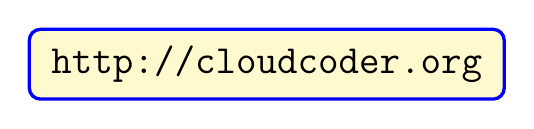
\begin{tikzpicture}
%        \Large\url{http://cloudcoder.org}
        \node [bigurl] {{\Large\tt http://cloudcoder.org}};
      \end{tikzpicture}
    }
  }

  \headerbox{Programming exercises!}{name=exercises,column=0,below=tldr}{
    \vskip .1in
    {\raggedright\normalsize
    \BI
    \item Automatically-evaluated exercises are useful in introductory
          programming courses
      \BI
      \item For learning {\bf syntax}
      \item For learning {\bf basic concepts}
            (variables, decisions, loops, etc.)
      \item For extra {\bf practice}
      \item For {\bf assessment}
      \EI
    \item They can be {\bf incorporated easily} into an existing
          course {\bf without major changes}
      \BI
      \item Use them to supplement readings, for quizzes,
            for practice, etc.
      \EI
    \EI
    }
  }

  \headerbox{We need another system?}{name=anothersystem,column=0,below=exercises}{
    \vskip .1in
    {\raggedright\normalsize
    \BI
    \item Many {\bf existing systems}:
          CodingBat, PracticeIt!, CodeLab, etc.
    \item We didn't know of one which
      \BI
      \item Was {\bf open source}
      \item Was {\bf community-supported}
      \item Had {\bf freely-redistributable exercises}
      \item Allowed self-hosting and {\bf full access to
            student data}
      \item Supported {\bf in-class assessment} (i.e., quizzes)
      \item Supported C/C++
      \EI
    %\item So we wrote one
    \EI
    }
  }

  \headerbox{Requirements}{name=requirements,column=1}{
    \vskip .1in
    {\raggedright\normalsize
    \BI
    \item Students need {\bf just a web browser}
      \BI
      \item {\bf No plugin} required: client is 100\% HTML/CSS/Javascript
      \EI
    \item System runs on {\bf two Linux servers}
      \BI
      \item One (network-facing) for webapp and database:
            EC2 micro instance works well
      \item One (network connected) to build and test submissions:
            can be any PC connected to network
      \EI
    \item Relatively easy installation
    \EI
    }
  }

  \headerbox{Need for a community}{name=community,column=1,below=requirements}{
    \vskip .1in
    {\raggedright\normalsize
    \BI
    \item Thesis: for a programming exercise system
          to be as useful as it can be, it needs a {\it community}
      \BI
      \item To {\bf provide exercises} that can be freely
            reused and improved
      \item To {\bf share experience} about how to use
            exercises most effectively
      \EI
    \EI
    }
  }

  \headerbox{Exercise repository}{name=repository,column=1,below=community}{
    \vskip .1in
    {\raggedright\normalsize
    \BI
    \item Writing good exercises is a challenge:
          but {\bf many hands make light work}
    \item CloudCoder {\bf exercise repository}:\\
          \url{https://cloudcoder.org/repo}
      \BI
      \item {\bf User-contributed} exercises
      \item All exercises available under {\bf permissive licenses}
            (Creative Commons or GNU FDL)
      \EI
    \item Can we add {\bf social features} to the
          exercise repository to allow users
          to
      \BI
      \item {\bf Classify} exercises? (tagging)
      \item {\bf Rate} exercises?
      \item Fork and {\bf improve} existing exercises?
      \item {\bf Recommend} exercises?
      \item Recommend {\bf sequences} of exercises?
      \EI
%          Goal: implement these features
%          by August 2013
    \EI
    }
  }

  \headerbox{Screenshots}{name=screenshot,column=2,span=3}{
    \vskip .1in
    \begin{minipage}[t]{4.5in}
    \centerline{\bf\underline{Main menu, choosing an exercise}}
    \vskip .1in
    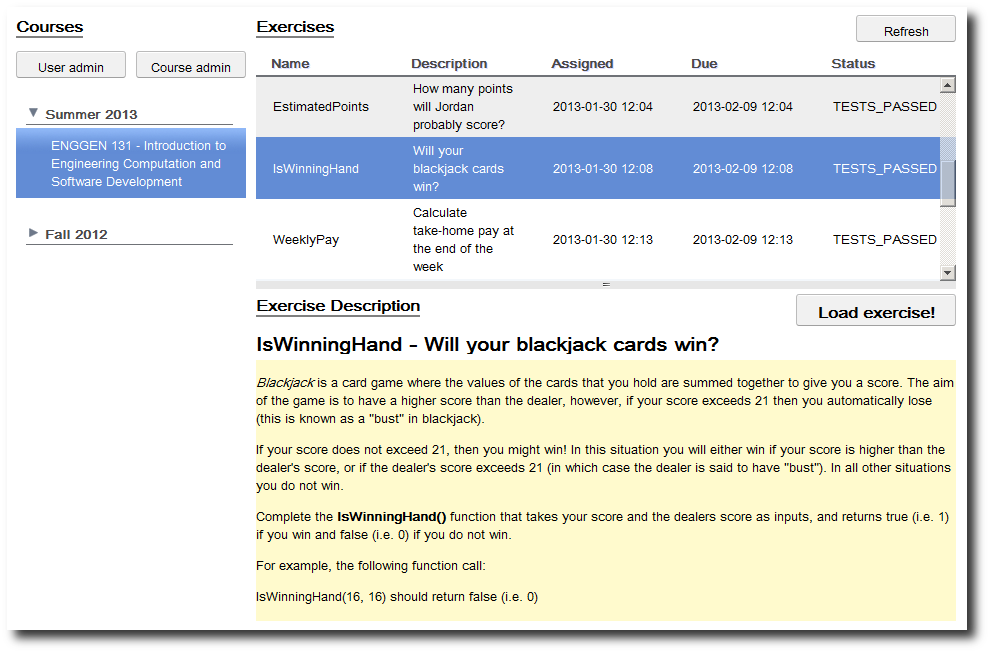
\includegraphics[height=3in]{images/menu}
    \end{minipage}\hskip .3in\begin{minipage}[t]{4in}
    \centerline{\bf\underline{Working on an exercise}}
    \vskip .1in
    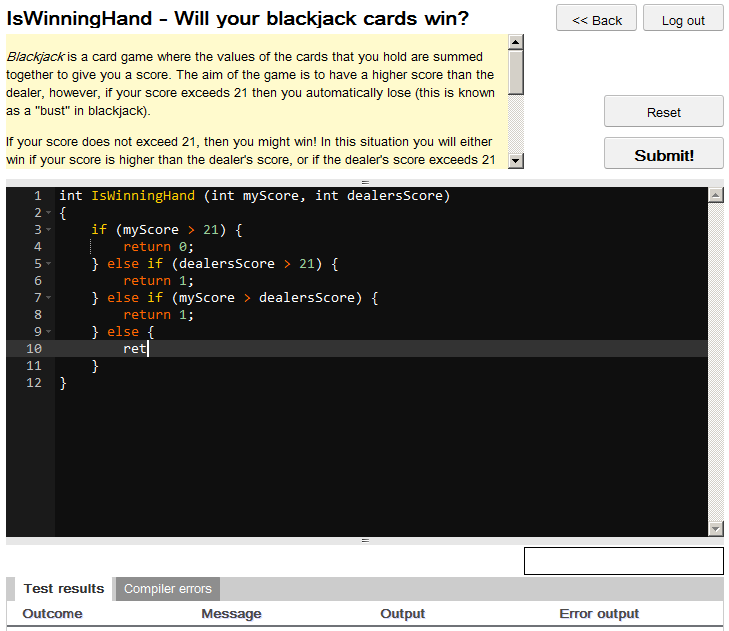
\includegraphics[height=3in]{images/exercise}
    \end{minipage}
    
  }

  \headerbox{Research questions}{name=questions,column=2,span=2,below=screenshot}{
    \vskip .1in
    \begin{minipage}[t]{2.8in}
    {\raggedright\normalsize
    \BI
    \item Can we detect students who are ``flailing''?
    Consider student A:
    \vskip .1in
    \centerline{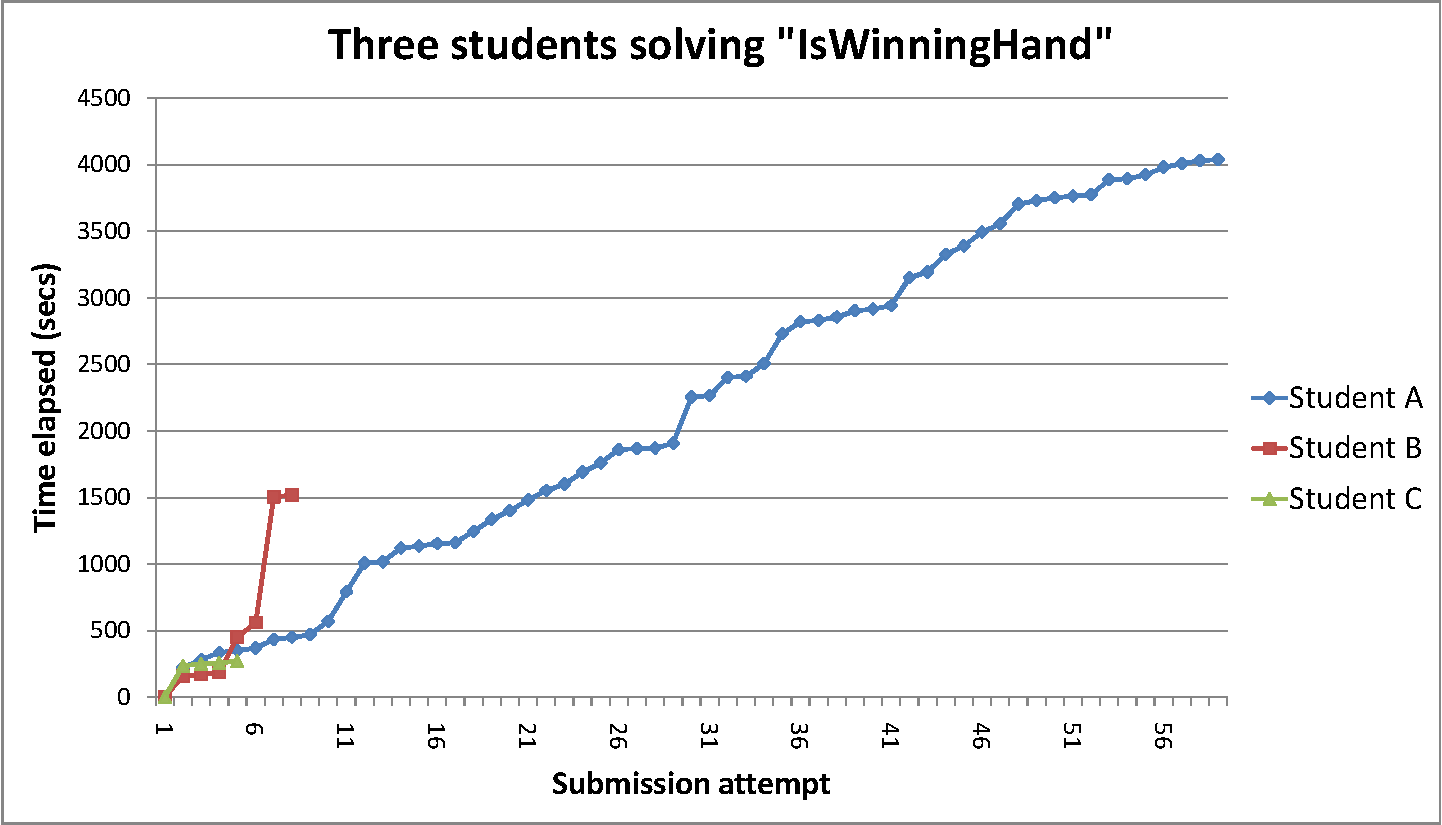
\includegraphics[width=2.3in]{images/Comparison}}
    \item Are exercises an effective ``prescription'' for
          students who are struggling?
    \item How can we motivate students to do practice problems?
      \BI
      \item Badges? Other forms of rewards/encouragement?
      \EI
    \item What are student perceptions of exercises?
    \item Can exercises be reused effectively?
      \BI
      \item In different courses?
      \item At different institutions?
      \EI
    \EI
    }
    \end{minipage}\hskip .1in\begin{minipage}[t]{2.8in}
    {\raggedright\normalsize
    \BI
    \item Do we see improved outcomes when students do exercises?
    \vskip .1in
    \centerline{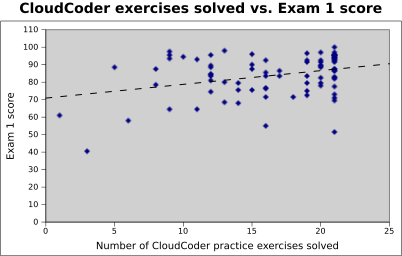
\includegraphics[width=2.2in]{images/exam1correlation}}
    \vskip .1in
    Moderate ($r \approx 0.33$) correlation between number of CloudCoder practice
    exercises solved and score on Exam 1 (variables, expressions,
    decisions, and loops) in CS 101 at York College, Spring 2013
    \EI
    }
    \end{minipage}
  }

  \headerbox{Conclusions, future work}{name=futurework,column=4,below=screenshot}{
    \vskip .1in
    {\raggedright\normalsize
    \BI
    \item Future work?
    \EI
    }
  }

  \headerbox{References}{name=references,column=4,below=futurework}{
    \vskip .1in
    {\raggedright\normalsize
    References?
    }
  }

  \headerbox{Support}{name=support,column=4,below=references}{
    \vskip .1in
    {\raggedright\normalsize
    Supported by a SIGCSE special projects grant, May 2012
    }
  }

\end{poster}

\end{document}
